\documentclass[a4paper,11pt,titlepage]{article}
\usepackage[utf8]{inputenc}
\usepackage{lmodern}
\usepackage[T1]{fontenc}
\usepackage[babel=true]{microtype}
\usepackage[portuguese]{babel}
\usepackage[pdftex]{hyperref}
\usepackage{graphicx}
\usepackage{eurosym}
\usepackage{scrextend}
\usepackage{hyphenat}
\usepackage{url}
\usepackage{hyperref}
\usepackage{float}

\title{\huge \textbf{Cage\\[1cm] \Large Relatório intercalar\\[0.7cm]

\includegraphics{res/logo.png}\\[0.7cm] \large Programação em
Lógica\\[0.25cm] \small $3^o$ ano\\[0.05cm]Mestrado Integrado em Engenharia Informática e
Computação\\[1cm]}\normalsize Turma 4 - Grupo Cage\_2}

\author{José Peixoto \\Luís Cruz \and 200603103\\201303248 \and ei12134@fe.up.pt
\\ up201303248@fe.up.pt}

\begin{document}
\maketitle

\section{Descrição do jogo}
O Cage é um jogo de estratégia em tabuleiro semelhante às damas que foi inventado por Mark Steere em maio de 2010. O autor descreve-o como um jogo para dois jogadores sem qualquer informação oculta. É abstrato e sem fator sorte, sem empates e sem temas. É jogado num tabuleiro de damas 10x10 ou 8x8 e, ao contrário do jogo original das damas, todo tabuleiro está preenchido, no início, com peças já promovidas a ``damas''. ``Jogo de aniquilação de alta energia'' é a frase escolhida pelo autor para caricaturar o jogo, uma vez que o movimento para o centro do tabuleiro assegura a aniquilação, de pelo menos, uma das cores.

\subsection{Regras}
O Cage é jogado por dois jogadores num tabuleiro de damas com 50 damas vermelhas e 50 damas azuis na versão de tabuleiro 10x10 ou com 32 damas vermelhas e 32 damas azuis na versão de 8x8 tabuleiro. O tabuleiro é iniciado preenchendo todas as casas com damas de cor alternada.

\subsubsection{Objetivo}
Para vencer é necessário capturar todas as damas inimigas. No final, pode ganhar-se mesmo que se perca a última peça que se está a movimentar (saltar) para capturar todas as damas inimigas ainda em jogo.

\subsubsection{Movimentos}
Existem quatro tipos de movimentos:
\begin{enumerate}
  \item Restrito
  \item Centralizador
  \item Adjacente
  \item Salto
\end{enumerate}
Durante um turno, um jogador apenas pode utilizar um tipo de movimento.

\paragraph{Restrição 1}
Nunca se pode colocar uma dama ortogonalmente (horizontal ou verticalmente) adjacente a uma dama de cor idêntica. Nem de forma transitória durante um turno de vários movimentos.

\paragraph{Restrição 2}
Nunca se pode movimentar uma dama que tenha adjacências ortogonais com damas inimigas para uma casa onde tal não aconteça.

\paragraph{Centralizador}
Este movimento de uma casa, permite à dama deslocar-se na horizontal, vertical ou diagonal para uma casa vazia e que permite que a dama se aproxime do centro do tabuleiro.


\paragraph{Adjacente}
Uma dama que não tenha adjacências ortogonais com damas inimigas pode mover-se apenas uma casa em qualquer direção que contenha adjacências ortogonais com uma ou mais damas inimigas.

\paragraph{Salto}
O movimento de salto permite capturar uma dama inimiga, movimentando a dama do jogador de uma casa ortogonalmente adjacente de um lado da dama inimiga para a casa vazia adjacente do lado oposto. É possível capturar uma dama inimiga nas casas periféricas do tabuleiro de uma casa adjacente e do lado oposto da dama inimiga na borda do tabuleiro. O resultado é que quer a dama capturada quer a dama que captura são removidas do tabuleiro.

\section{Representação do estado do jogo}
\iffalse (tipicamente uma lista de listas que incluem diferentes átomos para as peças), com exemplificação em Prolog de estados iniciais, intermédios e finais do jogo, acompanhados de imagens ilustrativas \fi
Na representação de jogo usar-se-ão listas de listas que apenas incluem
átomos para os diferentes tipos de peças ($red$ e $blue$) e a casa vazia ($empty$).
\subsection{Representação do estado inicial do tabuleiro:}
\begin{verbatim}
[[blue,red,blue,red,blue,red,blue,red],
 [red,blue,red,blue,red,blue,red,blue],
 [blue,red,blue,red,blue,red,blue,red],
 [red,blue,red,blue,red,blue,red,blue],
 [blue,red,blue,red,blue,red,blue,red],
 [red,blue,red,blue,red,blue,red,blue],
 [blue,red,blue,red,blue,red,blue,red],
 [red,blue,red,blue,red,blue,red,blue]
]).
\end{verbatim}

\begin{figure}[H]
    \center
    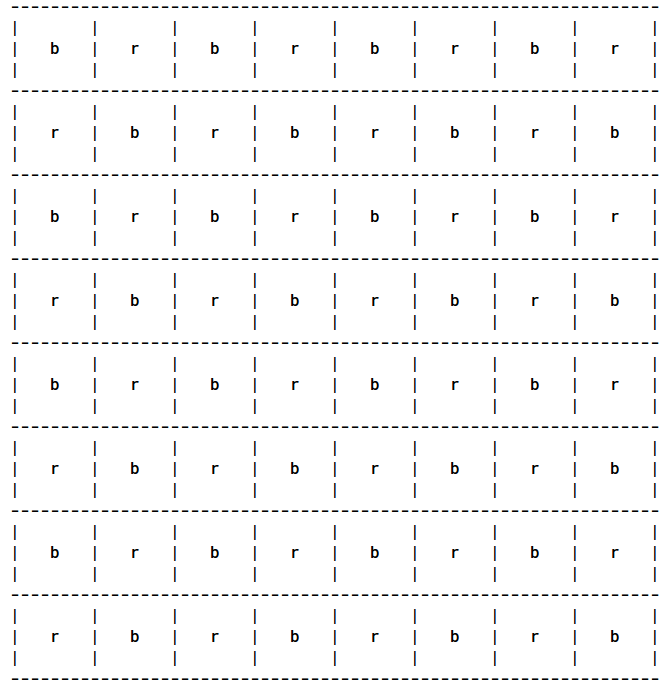
\includegraphics[scale=0.35]{res/initial-state-cli.png}
    \caption{Estado inicial do jogo (linha de comandos)}
    \label{fig:initial-state-cli.jpg}
\end{figure}

\begin{figure}[H]
    \center
    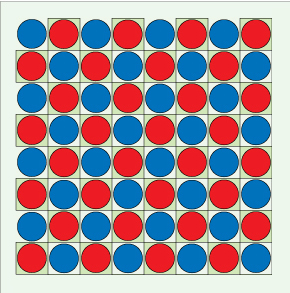
\includegraphics[scale=0.8]{res/initial-state.jpg}
    \caption{Estado inicial do jogo}
    \label{fig:initial-state.png}
\end{figure}

\subsection{Representação de um estado intermédio do tabuleiro:}
\begin{verbatim}
[[empty,empty,empty,empty,empty,empty,empty,empty],
 [empty,empty,empty,empty,empty,empty,empty,empty],
 [empty,empty,empty,empty,empty,empty,empty,empty],
 [empty,red,blue,empty,empty,empty,empty,empty],
 [red,empty,empty,empty,empty,empty,empty,empty],
 [empty,blue,empty,empty,empty,empty,empty,empty],
 [empty,empty,empty,empty,empty,empty,empty,empty],
 [empty,empty,empty,empty,empty,empty,empty,empty]
]).
\end{verbatim}

\begin{figure}[H]
    \center
    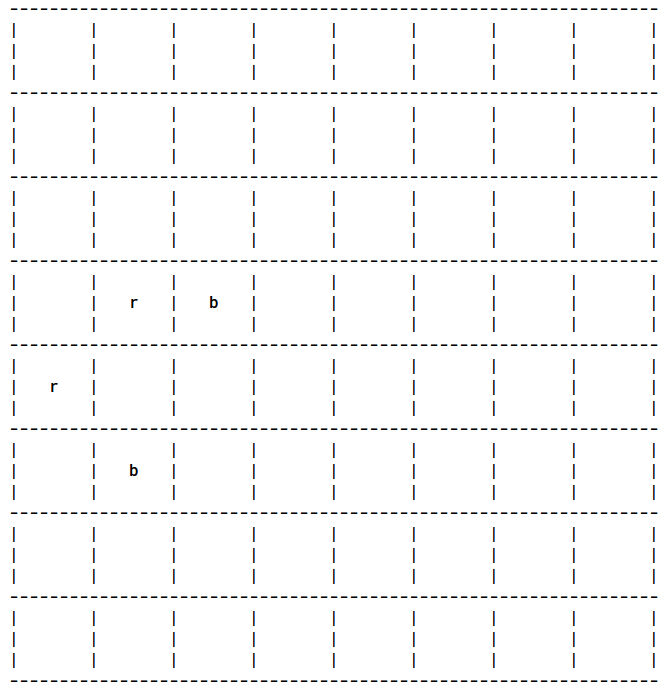
\includegraphics[scale=0.35]{res/intermediate-state-cli.png}
    \caption{Estado intermédio de um jogo (linha de comandos)}
    \label{fig:intermediate-state-cli.png}
\end{figure}

\begin{figure}[H]
    \center
    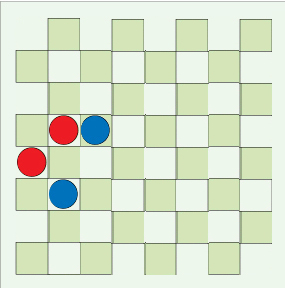
\includegraphics[scale=0.8]{res/intermediate-state.jpg}
    \caption{Estado intermédio de um jogo}
    \label{intermediate-state.jpg}
\end{figure}

\subsection{Representação de um possível estado final do tabuleiro:}
\begin{verbatim}
[[empty,empty,empty,empty,empty,empty,empty,empty],
 [empty,empty,empty,empty,empty,empty,empty,empty],
 [empty,empty,empty,empty,empty,empty,empty,empty],
 [empty,empty,empty,empty,empty,empty,empty,empty],
 [empty,empty,empty,empty,empty,empty,empty,empty],
 [empty,empty,empty,empty,empty,empty,empty,empty],
 [empty,empty,empty,empty,empty,empty,empty,empty],
 [empty,empty,empty,empty,empty,empty,empty,empty]
]).
\end{verbatim}

\begin{figure}[H]
    \center
    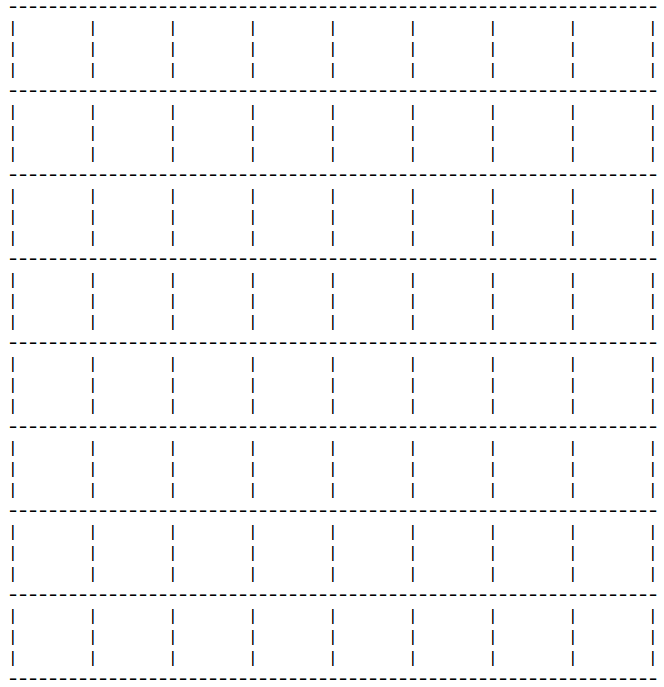
\includegraphics[scale=0.36]{res/final-state-cli.png}
    \caption{Estado final de um jogo CLI (linha de comandos)}
    \label{fig:final-state-cli.png}
\end{figure}

\begin{figure}[H]
    \center
    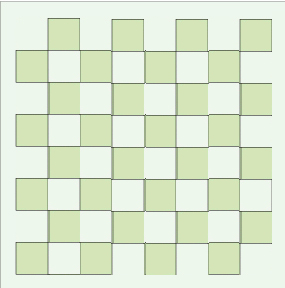
\includegraphics[scale=0.8]{res/final-state.jpg}
    \caption{Estado final de um jogo}
    \label{final-state.jpg}
\end{figure}

\section{Visualização do tabuleiro em modo de texto}
\iffalse (tipicamente uma lista de listas que incluem diferentes átomos para as peças), com exemplificação em Prolog de estados iniciais, intermédios e finais do jogo, acompanhados de imagens ilustrativas \fi
\begin{verbatim}
% container
board([[blue,red,blue,red,blue,red,blue,red],
       [red,blue,red,blue,red,blue,red,blue],
       [blue,red,blue,red,blue,red,blue,red],
       [red,blue,red,blue,red,blue,red,blue],
       [blue,red,blue,red,blue,red,blue,red],
       [red,blue,red,blue,red,blue,red,blue],
       [blue,red,blue,red,blue,red,blue,red],
       [red,blue,red,blue,red,blue,red,blue]
      ]).

% display board
display_board([H|T]) :- 
        % how to display 1st line border?
        write('   -------------------------------------------- '), nl,
        display_empty_line([]),
        display_line(H), nl,
        display_empty_line([]),
        display_board(T).

display_board([]):-
        write('   -------------------------------------------- '), nl.

% display line
display_line([H|T]) :-
        symbol(H,S),
        write('   |   '), write(S), 
        display_line(T).
display_line([]) :-
        write('   |   ').

%display empty line
display_empty_line([]):-
        write('   '), write('|'),write('       '),
        write('|'), write('       '), write('|'),
        write('       '), write('|'), write('       '),
        write('|'), write('       '), write('|'), write('       '),
        write('|'), write('       '), write('|'), write('       '),
        write('|'), nl.

% symbols
symbol(red,'r').
symbol(blue,'b').
symbol(empty,' ').
\end{verbatim}

\section{Movimentos}
\iffalse (tipos de jogadas) possíveis, definindo os cabeçalhos dos predicados que serão depois implementados. \fi
De uma forma geral, nos predicados dos movimentos a seguir apresentados, é requerida a receção das linhas e colunas iniciais e finais da peça a mover e do tabuleiro.
\subsection{Restrições}
Restrições aos predicados dos movimentos declarados a seguir. Presume-se que a implementação dos outros predicados relativos aos restantes movimentos requeiram a avaliação satisfatória das seguintes restrições.
\begin{verbatim}
restriction_1(row,col,adj_row,adj_col,boad).
restriction_2(row,col,adj_row,adj_col,board).
\end{verbatim}

\subsection{Centralizador}
Cabeçalho do predicado do movimento que centraliza a dama ao centro do tabuleiro.
\begin{verbatim}
centering_move(row,col,dest_row,dest_col,board).
\end{verbatim}

\subsection{Adjacente}
Cabeçalho do predicado do movimento para uma casa adjacente.
\begin{verbatim}
adjoining_mode(row,col,dest_row,dest_col,board).
\end{verbatim}

\subsection{Salto}
Cabeçalho do predicado do movimento em salto que permite capturar damas inimigas.
\begin{verbatim}
jump(row,col,dest_row,dest_col,board).
\end{verbatim}


\begin{thebibliography}{9}
\bibitem{lamport93}
  Sterling, Leon
  \emph{The Art of Prolog},
  The MIT Press
  2nd edition,
  2000.
  
  \bibitem{bl}Abstract games,
  \url{http://www.marksteeregames.com/MSG_abstract_games.html}, 14 10 2016.
  
  \bibitem{bl}Cage rules,
  \url{http://www.marksteeregames.com/Cage_rules.html}, 14 10 2016.
\end{thebibliography}

\end{document}

